\documentclass[preprint]{elsarticle}
\usepackage{fullpage, graphicx,subfigure,multirow}
\journal{JAC}
\biboptions{sort&compress,comma,square}
\usepackage{color}
\usepackage{fullpage,subfigure,caption,float,psfrag}
\usepackage[bookmarks=true,pdftoolbar=true]{hyperref}
\hypersetup{%
  pdftitle = {Structural transformations in Co - Al SMA's},
  pdfkeywords = {pdf, hyperref, bookmarks},
  pdfauthor = {Anjana Talapatra}}
\usepackage[all]{hypcap}
\usepackage{dcolumn}
\usepackage{bm}
\usepackage{xspace}   
\usepackage{siunitx,cleveref,stmaryrd}

 
\begin{document}

\begin{frontmatter}

\title{Investigation of the energetics of structural transformations in Co-based binary alloys }
 
\author[meen]{Anjana Talapatra\corref{cor1}}
\ead{anjanatalapatra@tamu.edu}
\author[msen]{Raymundo Arr\'{o}yave}


\cortext[cor1]{Corresponding address: Mail Stop 3123, Texas A$\&$M University, College Station, TX 77843-3123, United States}

\address[meen]{Department of Mechanical Engineering, Texas A$\&$M University, College Station, TX 77843-3123, United States}

\address[msen]{Department of Materials Science and Engineering , Texas A$\&$M University, College Station, TX 77843-3123, United States}

\begin{abstract}
The energy pathways associated with the martensitic transformation in shape memory alloys (SMA's), though the focus of extensive research over the past decades, are still unclear. In this work we build a framework using an energetics approach to describe the  martensitic  f.c.c-h.c.p transformation in Co-based alloys and to investigate the effect of alloying on the transformation  First principle calculations are used to determine the energy landscape of the transformation using the Shoji - Nishiyama and Wentzcovitch - Lam models in Co - (Al, Fe, Si) binary alloys over a range of composition. The martensitic transformation is an energy barrier crossing event and exhibits concomitant reduction in symmetry. Hence a steepest descent optimization technique is employed to realize the minimum energy path and the transition states of the transformations over the energy landscape. The energy barriers as a function of composition are  calculated  and compared against available  experimental data. 
\end{abstract}
\end{frontmatter}

%----------------------------------------------------------------------------------------------------------------------------------------------------------------------------------------------------------------------%
\section{Introduction}
\label{Sec:intro}

Nearly all phase transformations in solid metals and alloys are heterogeneous processes and can be classified as i) reconstructive and ii) displacive transformations \cite{christian2002theory}. In reconstructive transformations, bonds are broken and reformed to form the new phase. They encompass a change in the primary coordination and the transformed phase not a subgroup of parent phase and there is no associated energy barrier. Displacive transformations, on the other hand, occur by the ordered and correlated motions of atoms accompanied by a change in the  secondary
coordination. The transformed phase in this case is a subgroup of parent phase. The transition is of first order and is a barrier-overcoming process. Displacive martensitic transformations thus have an associated energy barrier which characterizes them. The energy barrier indicates the energy required for the transformation to occur and thereby is indicative of the martensitic transformation temperature. 

Pure cobalt shows a non-thermoelastic reversible martensitic transformation from a parent face centered (f.c.c - $\gamma$) phase to a hexagonal close packed 
(h.c.p - $\epsilon$) phase at $\simeq 695 \si{\kelvin} $\cite{koval2000high}. The transformation is accompanied by small changes in enthalpy
 ($\Delta h= 473 \si{\joule\per\mole}$) and volume ($\Delta V/V=3.3\times 10^{-3} $) and a sharp singularity of the specific heat,  attesting to it being a 
first order transformation \cite{toledano2001theory}. The system has a thermal hysteresis associated with it 
( $\approx 100 \si{\kelvin}$) which is quite high when compared with conventional thermoelastic SMA's. A number of factors affect the transformation temperature, 
such as grain size, purity, external stresses and alloying \cite{koval2000high}. Binary alloying drastically affects the transformation temperature in these alloys, as zirconium and 
molybdenum cause a reduction in the martensitic start temperature ($M_s$) with increased alloying while germanium and silicon additions result in an increase 
in $M_s$. Addition of aluminium or nickel do not affect the transformation temperature significantly\cite{koval2000high,omori2003}.

In 2003, Omori et al.\cite{omori2003} showed that addition of aluminium to cobalt promotes $L1_{2}$ ordering and thereby improves the reversibility of the 
transformation. The solubility of Al in Co is $\approx$ 16\% and the alloying does not reduce the ductility of the material. Consequently, Co - Al is a potential high temperature SMA (HTSMA) with high thermal stability. 

A number of attempts have been made to model the f.c.c-h.c.p phase transformation.The majority of these models describe the transition in terms of nucleation and
growth processes and the propagation of partial dislocations\cite{christian1951theory,basinski1953martensitic,bollmann1961phase}.  The other class of models are 
phenomenological models based on shearing mechanisms formulated by the decomposition of the distortion into two configuration co-ordinates. 
The Shoji - Nishiyama \cite{nishiyama1978} mechanism was the earliest such model which described a way of continuously distorting the f.c.c structure 
into a h.c.p structure using the simple hexagonal (s.h) reference structure, specifically for the transformation in cobalt alloys. More recently, Wentzcovitch et al. \cite{wentzcovitch1991fcc} proposed a parametric 
model to describe this transformation using an orthorhombic reference structure. As mentioned above, the martensitic transformation in cobalt is a displacive transformation accomplished
by the cooperative movement of atoms while maintaining the primary co-ordination and thereby lends itself well to analysis using parametric models.   In this work, the martensitic transformations in Co-based binary alloys are investigated 
using the two phenomenological models described above using ab-initio methods within a DFT framework with a view to assessing the effect of alloying on the 
energetics of the transformation. Kibey at al\cite{kibey2009} use a similar process to model the $B2-B19' $ transformation in Ni-Ti.

These models yield the energy landscapes for the transformations given the initial and final structures. For transformations with relatively smooth energy surfaces,the  most probable pathways are the minimum energy paths (MEP). Minimum energy paths have physical significance  in the low temperature behavior  of a system as they give insight into the
energy barrier involved in a thermally activated event (phase transformation)  without any inputs about  the width of the channel near the saddle point or other effects due to entropy. The energy surfaces calculated in this work are a result of ground state calculations and hence are sufficiently smooth to bear relevance for MEP calculations. 
At high temperature, thermal fluctuations cause the energy surface  to lose smoothness and multiple energy peaks of  the order of kBT  make the concept of the MEP irrelevant. However at high temperatures,  the MEP will  still correspond to the path with the maximum likelihood.
Thus the problem reduces to obtaining the MEP over a energy surface when the initial and final states are known. The techniques used for such scenarios include the string method\cite{qian2005current, samanta2010modified} and the nudged elastic band(NEB)\cite{jonsson1998nudged} methods. In this work we use the string method as implemented by Samanta et al. \cite{samanta2010modified} to determine the MEP for the transformations.

The objective of this work is to build a framework to assess the viability of martensitic transformations in Co-based binary alloys from an energetics
 point of view, to investigate the effect of Al alloying on the transformation and finally,to extend the framework to allow investigations
on ternary Co - Al based alloys. Additionally, the framework may be used to study other SMA's which show similar transformations.

The organization of this article is as follows. In Section \ref{Sec:bain} we debate the applicability of the Bain transition mechanism in the case of Co-based alloys and show 
the energetics of the Bain path in the Co - Al system. In Section \ref{Sec:fcc_hcp} the phenomenological models for the f.c.c to h.c.p transformation are discussed and applied to the binary
 Co - Al, Co-Si and Co-Fe binary alloys by extending the ideas presented in \cite{wentzcovitch1991fcc, folkins1990configuration}  . In Section \ref{Sec:results} the minimum energy paths for the transformations are realized using a steepest descent algorithm and the results are
compared with experimental data. An attempt is made to provide a theoretical basis for the minimum energy paths obtained. Finally, in Section \ref{Sec:summary} we 
summarize our results and conclude by delineating the characteristics of the martensitic transformation in Co-based alloys.

%----------------------------------------------------------------------------------------------------------------------------------------------------------------------------------------------------------------------%
\section{f.c.c - b.c.c transformation}
\label{Sec:bain}
\begin{figure}[ht]
  \centering
  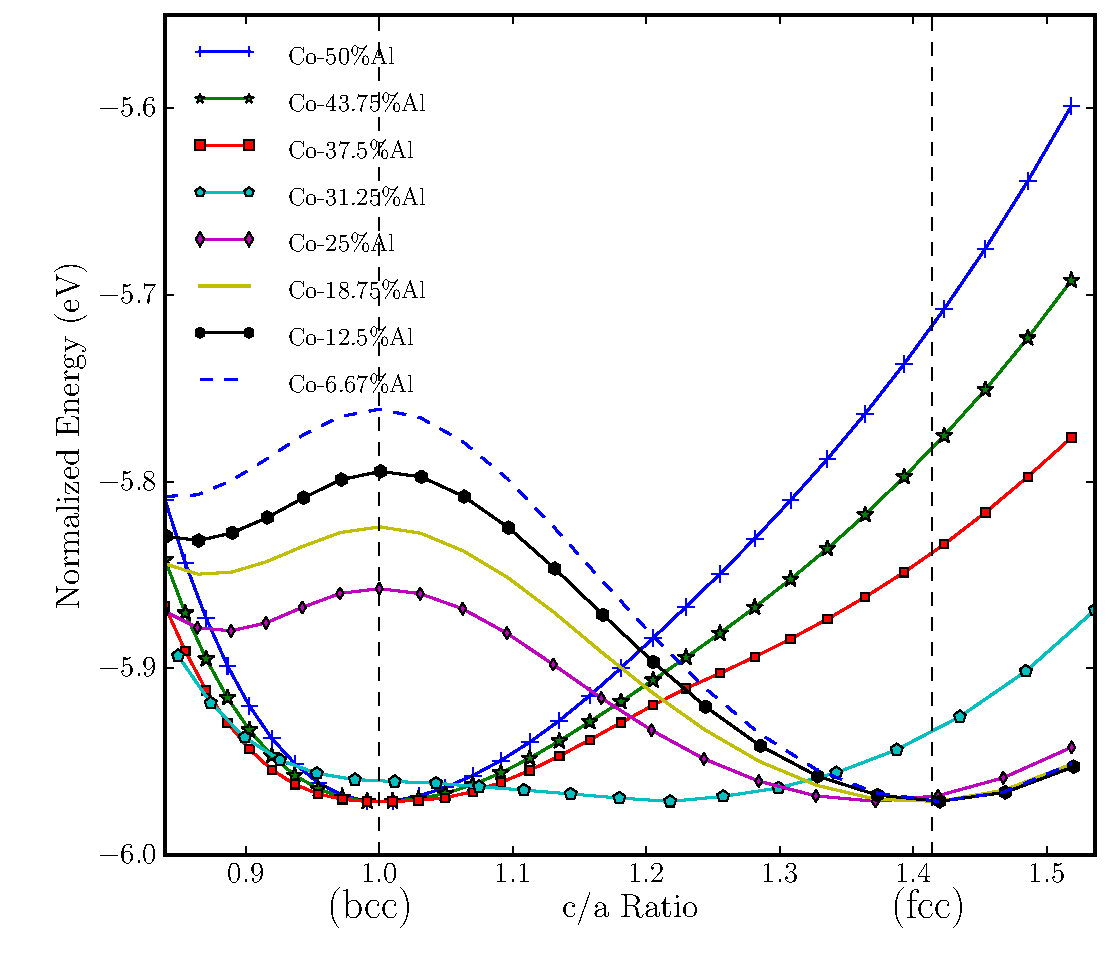
\includegraphics[scale = 0.6]{figure_1}
  \caption{Bain path in Co - Al for alloying up to 50\% Al}
  \label{fig:CoAl_bain}
\end{figure}

Cobalt is the only element displaying a f.c.c-h.c.p transition which does not possess a disordered body centered (b.c.c) phase in it's phase diagram. In elements which do possess the b.c.c phase,  the f.c.c and h.c.p structures can be attained from the  parent bcc structure via the Bain\cite{bain1924}  and Burgers\cite{Burgers1934} transformations. The Co - Al phase diagram however, shows a bcc phase at compositions greater than around 25 \% Al. To validate the use of these distortion models,the phase stability of competing phases was studied by carrying out Bain path calculations for the Co - Al system for up to Co-50 \% Al as shown in Fig. \ref{fig:CoAl_bain}.
\textcolor{red}{The Bain transformation can be described as a tetragonal distortion of the cubic austenitic phase. If one assumes that the transformation occurs with minimal volume change, then it can be described through the Bain path, which essentially transforms a bcc structure into a fcc variant as the c/a ratio of the lattice goes from 1 to $\sqrt{2}$. We used a 16 atom supercell to model the Bain path for the various compositons. For each composition, calculations were carried out by positioning alloying element in 3 different configurations. Results did not differ significantly hence structure yielding the lowest energy was chosen and used for the calculations.
The calculations were performed within the framework of density functional theory, as implemented in the Vienna ab initio simulation package (VASP)\cite{kresse1996software}, applying the generalized gradient approximation (GGA) using the Perdew-Wang 1991 (PW91) functional \cite{Perdew1992}.  The electronic configurations of the relevant elements were realized using  the projector augmented wave (PAW) pseudo-potentials formalism \cite{blochl1994paw}. Brillouin zone integrations were performed using a Monkhorst-Pack mesh \cite{monkhorst1976} with at least 5000 $k$ points per Brillouin zone or cell. Full relaxations for the cubic structures were realized by using the Methfessel-Paxton smearing method of order 1 \cite{methfessel1989}, and self-consistent static calculations were carried out  with the tetrahedron smearing method with Bl\"{o}chl  corrections \cite{blochl1994improved}. A cutoff energy of 350 eV was used for all the  Bain path calculations and spin polarizations were accounted for as well. The energy cutoff is more that 30 \% of the recommended energy cutoff for each of the consitutuent elements. Convergence of the electronic structure was assumed, when changes between two consecutive steps fell below $10^{-7} eV$.}

It is seen that the Co - Al system shows a minima  at a c/a ratio of $\approx$ 1.43 up to Co-25\% Al. Beyond 25\% Al there is a sharp shift in the stability and the bcc structure (c/a = 1) is stabilized for increasing amounts of Al, which agrees with the Co - Al phase diagram in that this system is dominated by a B2 - ordered phase close to the 1:1 stoichiometry. While the Bain path is not relevant to the problem at hand, the fact that it's composition dependence closely mirrors the expected topology of the binary phase diagram constitutes an indirect validation of the accuracy of the calculations.
%----------------------------------------------------------------------------------------------------------------------------------------------------------------------------------------------------------------------%
 \section{f.c.c - h.c.p transformation}
\label{Sec:fcc_hcp}
It is well established experimentally that Co - Al alloys show a f.c.c - h.c.p transformation with a good shape memory effect for Al $>$ 10\%.\cite{omori2003}.
On an atomic level, the martensitic transformation is realized by a combination of finite displacements (shuffles) along various directions. 
However, the energy path associated with this transformation has not been previously examined to the best of the authors knowledge. This work explores the energy surface associated with the f.c.c - h.c.p transformation
in Co - Al via two mechanisms mentioned in section \ref{Sec:intro}: the conventional Shoji- Nishiyama path \cite{nishiyama1978} and the recent mechanism presented by Wentzcovitch et. al. \cite{wentzcovitch1991fcc}.

\subsection{Shoji-Nishiyama (SN) path for the f.c.c-h.c.p transformation in Co - Al}

The SN path models a continuous distortion of the parent f.c.c phase into the h.c.p phase which can be visualized by a decomposition into two configurational 
co-ordinates as proposed by Folkins and Walker\cite{folkins1990configuration}; one accounting for the shearing of the crystal and the other describing the relative 
sinusoidal displacements of atomic planes.The  planar correspondence is given by: $ (1 1 1)_{fcc} \parallel (0 0 0 1)_{hcp}$ , $ [1 1\bar2]_{fcc} \hspace{0.2em} 
\parallel [1\bar1 0 0]_{hcp}$ , or $ [1 \bar1 0]_{fcc} \parallel [1 1 \bar2 0]_{hcp}$.
This transformation occurs by shifting every other $ (1 1 1)$ f.c.c plane by $(a/6)[1 1\bar2]$.
 \begin{figure}[ht]
   \centering
   \subfigure[]{
       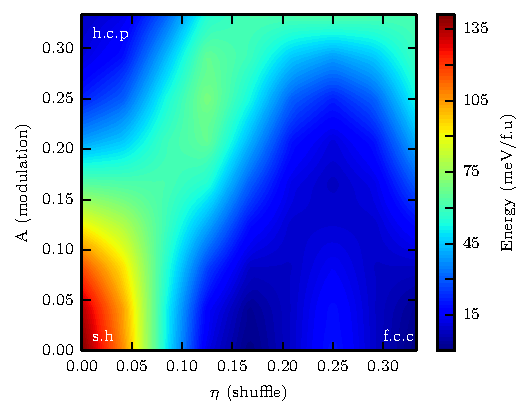
\includegraphics[scale=0.85]{figure_2a}
       \label{fig:SN_energy}
       }
 \subfigure[]{
       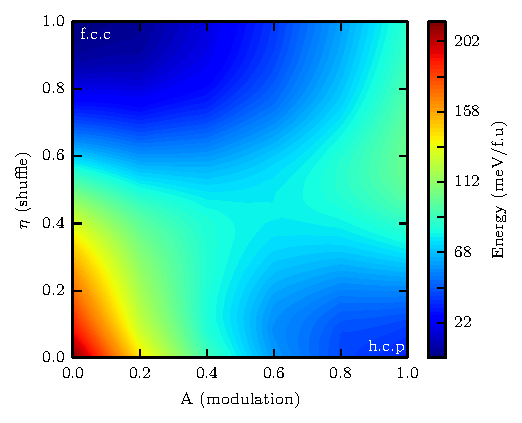
\includegraphics[scale=0.85]{figure_2b}
       \label{fig:SN_3D}
       }
\caption{a)Energy contour pure aluminium for the SN mechanism. (0,0) corresponds to the simple hexagonal (s.h) reference structure, ($0,\frac{1}{3}$) corresponds to the h.c.p structure while ($\frac{1}{3},0$) indicates the f.c.c structure. b)Energy contour for pure aluminium for the WL mechanism. (0,1)refers to the f.c.c structure while (1,0) describes the h.c.p 
structure.}
 \end{figure}
The parameterization of this transformation as formulated by Folkins and Walker  is used for the calculations. The formulation uses the simple hexagonal (s.h) structure as a 
reference structure, The f.c.c structure is then generated from the s.h structure by a shear along the $\hat{x}$ direction.The h.c.p structure is derived from the s.h structure by 
an alternating modulation along the $\hat{x}$ direction. For an atom with position vector 
$r=(x,y,z)$, it's displacement is then given by equation \ref{eqn:Shoji_Nishiyama}:
\begin{equation}
 u(A,\eta;r)=\eta \frac{3}{\sqrt{2}}z \hat{x} + A\frac{\sqrt{3}}{2} a\cos(Q.r)\hat{x}
\label{eqn:Shoji_Nishiyama}
\end{equation}
 with $Q=(\frac{\pi}{c})\hat{z}$.The $\eta$ term on the right hand side of the equation denotes the shear.It describes the lateral shearing of each hexagonal plane by $\eta \frac{3}{\sqrt{2}}z$.
The second term describes the modulation associated with the h.c.p structure. For further details regarding this formulation, refer to \cite{folkins1990configuration}.

\subsection{Wentzkovitch-Lam (WL) path for the f.c.c - h.c.p transformation in Co - Al}

The alternate model proposed by Wentzkovitch\cite{wentzcovitch1991fcc} assumes a correspondence between  $ (0 0 1)_{fcc}$ and  $ (0 0 0 1)_{hcp}$ planes. This is achieved by the simultaneous 
occurrence of four strains\cite{wentzcovitch1991fcc}; Shear in opposite directions of the A and B layers along $[1 0 0]_{fcc}$ or  $[0 1 0]_{fcc}$ , a macroscopic strain along 
$[1 0 0]_{fcc}$ or  $[0 1 0]_{fcc}$ , another macroscopic strain along $[0 0 1]_{fcc}$ and a compressive strain along $[0 1 0]_{fcc}$ or $[1 0 0]_{fcc}$.

Atomic Displacement of an atom at r(x,y,z) within this formulation is given by equation \ref{eqn:renata};
\begin{equation}
 u(A,\epsilon_x, \epsilon_y, \epsilon_z;r)=\epsilon_x x \hat{x}+\epsilon_y y \hat{y}+ A(1+\epsilon_y)\frac{a}{\sqrt{2}}cos(Q.r)\hat{y}+\epsilon_z z \hat{z} 
\label{eqn:renata}
\end{equation}
where $Q=(2\pi/L)\hat{z}$ and $L=\sqrt{2} a$. $(1+\epsilon_{x})+(1+\epsilon_{y})+(1+\epsilon_{z})=1$ for both structures which implies a volume invariance. For more details please refer to 
\cite{wentzcovitch1991fcc}.
As seen in the figure,(1,0) corresponds  to the h.c.p structure and (0,1) to the f.c.c structure.
The minimum energy path(MEP) for this mechanism was then calculated using the modified string method\cite{samanta2010modified}, which is indicated in figure \ref{fig:ren_MEP}.
\begin{figure}[ht]
   \centering
   \subfigure[]{
   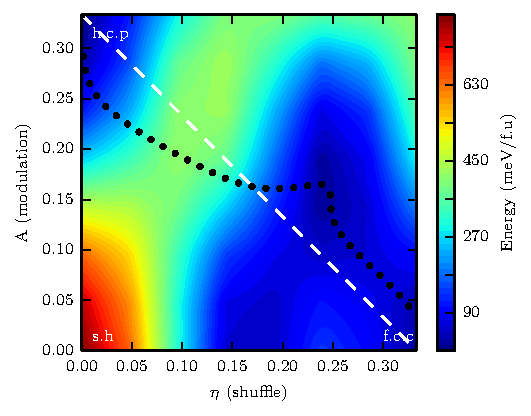
\includegraphics[scale=0.85]{figure_3a}
   }
   \subfigure[]{
   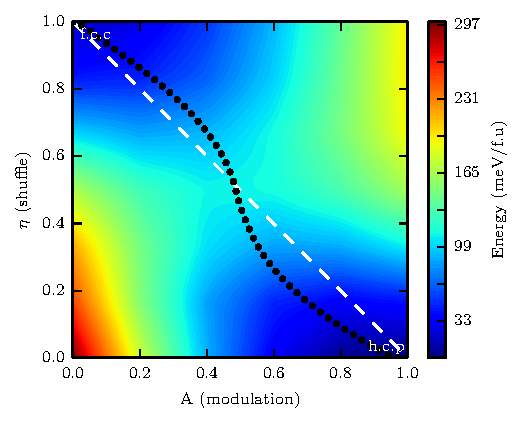
\includegraphics[scale=0.85]{figure_3b}
   }
   \caption{a)MEP calculated using the modified string method for pure cobalt for the SN mechanism. The
   dashed line indicates the initial straight line path while the  line with circular markers indicates the final optimized MEP. b) MEP calculated using the modified string method for pure cobalt for the WL mechanism. The
   dashed line indicates the initial straight line path while the solid line with circular markers indicates the final optimized MEP. }
   \label{fig:ren_MEP}
 \end{figure}
 %----------------------------------------------------------------------------------------------------------------------------------------------------------------------------------------------------------------------%
\section{Results and Discussion}
\label{Sec:results}
Calculations presented in this work  were performed within the framework of Density Functional Theory,
as implemented in the Vienna ab initio simulation package (VASP), applying generalized
gradient approximation (GGA) using the Perdew-Wang 1991 (PW91) functional\cite{Perdew1992}. The electronic configurations of the appropriate elements were realized using  the projector augmented-wave (PAW) pseudo-potentials formalism \cite{blochl1994paw}.Brillouin zone integrations were performed using a Monkhorst-Pack mesh \cite{monkhorst1976} with atleast 5000 k-points per reciprocal atom. Full relaxations were realized by using the Methfessel-Paxton smearing method of order one \cite{methfessel1989} and self-consistent static calculations were carried out  with the
tetrahedron smearing method with Bl\"{o}chl  corrections \cite{blochl1994improved}. A cutoff energy of 350 eV was used for all the calculations and spin polarizations were accounted for as well.The energy cutoff is more that 30 \% of the recommended energy cutoff for each of the consitutuent elements. 
The f.c.c - h.c.p transformation was modeled using the Wentzcovitch-Lam (WL) and the Shoji-Nishiyama (SN) mechanisms  for the Co - Al, Co-Fe and Co-Si systems. The results are presented below.
\begin{figure}[htp!]
    \centering
    \subfigure[]{
     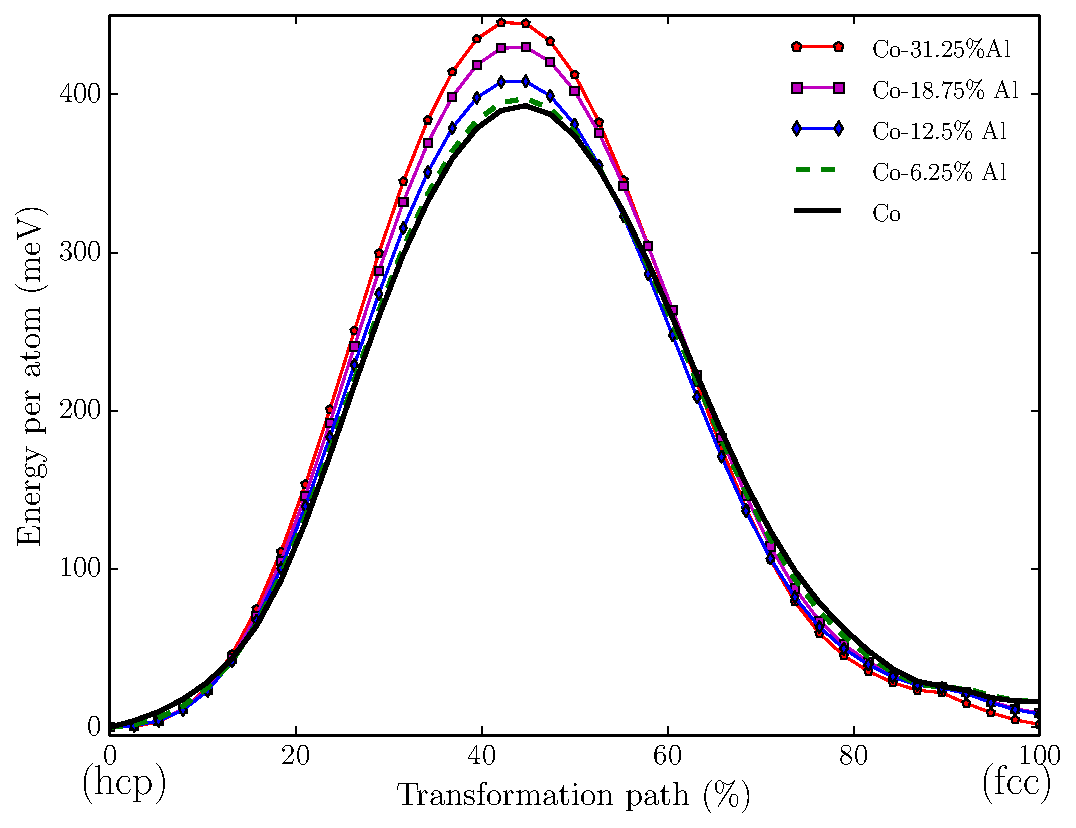
\includegraphics[scale=0.4]{figure_4a}
        \label{fig:Co_Al_sn}
        }
  \subfigure[]{
        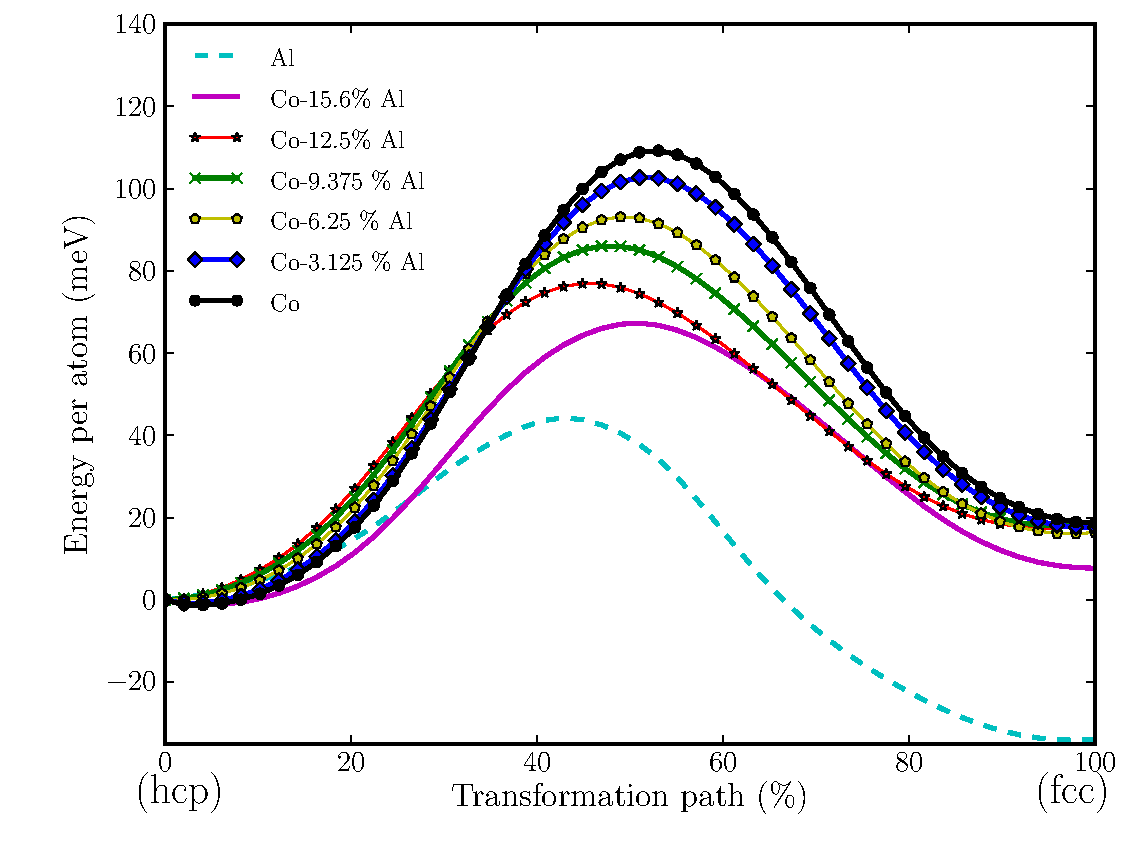
\includegraphics[scale=0.4]{figure_4b}
        \label{fig:Co_Al_ren}
        }
\caption{MEP profile for various compositions of Co - Al for the a) SN and b) WL mechanisms}
\label{fig:linear_profiles}
  \end{figure}    
%%%%%%%%%%%%%%%%%%%%%%%%%%%%%%%%%%%%%%%%%%%%%%%%%%%%%%%%%%%%%%%%%%    

This section shows the results obtained for the f.c.c. - h.c.p transformation paths using the WL and SN models. Calculations have been carried out for the Co - Al, Co-Fe and Co-Si systems. For both Al and Fe, experiments have shown that the martensitic transformation temperature of cobalt  is expected to decrease with increased alloying. The addition of Si shows the opposite effect, the martensitic tranformation temperature increases with increased alloying \cite{ma2010high}.

 \Cref{fig:Co_Al_ren} shows the MEP profiles for varying compositions of Co - Al and Figure \ref{fig:Co_Al_dE_ren} shows the trend observed in the energy barrier for the transformation for varying compositions of Co - Al using the WL model. 
 We see a reduction in the energy barrier (which indicates a lowering of $M_s$) for increasing amounts of Al, which is corroborated by experimental works\cite{omori2003} which indicate a lowering of the $M_s$ with addition of aluminium.  This trend stays the same throughout the range of composition for which calculations were carried out.
 
 \Cref{fig:Co_Al_sn} shows the MEP profiles for varying compositions of Co - Al  and Figure \ref{fig:Co_Al_dE_sn} shows the trend observed in the energy barrier for the transformation for varying compositions of Co - Al  for the Shoji-Nishiyama  model.
 The SN model shows a contrasting trend. We see an increase  in the energy barrier (which indicates an increase in  $M_s$) with increasing amounts of Al which is opposite to what is known experimentally. Additionally, the energy barriers calculated are also much higher than that for the WL model.

 A SN model with zero transformation deformation may also be formulated by considering a combination of deformations in the three equivalent shear directions\cite{nishiyama1978}. Planar shifts of $(a/6)[\bar2 1 1]$, $(a/6)[1 \bar2 1]$ on the $ (1 1 1)$ f.c.c plane are equivalent to $(a/6)[1 1\bar2]$. Each of these shifts causes a total shear of \ang{19.5}. If these three variants are stacked with equal thickness the resultant deformation shear will reduce to zero, i.e they will cancel each other in the bulk cell. This will mean a small resultant shear for the martensitic transformation and may result in an easier transformation. This model was also implemented for comparison and calculations were carried out for the Co - Al system.  
 \Cref{fig:Co_Al_sn_zero} shows the MEP profiles for varying compositions of Co - Al  and Figure \ref{fig:Co_Al_dE_sn_zero} shows the trend observed in the energy barrier for the transformation for varying compositions of Co - Al  for the modified zero transformation deformation Shoji-Nishiyama  model. Comparing figures \ref{fig:Co_Al_sn} and \ref{fig:Co_Al_sn_zero}, it is seen that while there is a reduction in the absolute values of the energy barrier for the transformation compared to the simple SN model, it is still much higher than for the WL model. Additionally, in figure \ref{fig:Co_Al_dE_sn_zero} we still see an increase in the energy barrier with addition of Al, contrary to experiments. Consequently, we do not use the zero deformation shear model for any further analysis.

\begin{figure}[htp!]%[!h]
    \centering
  \subfigure[]{
        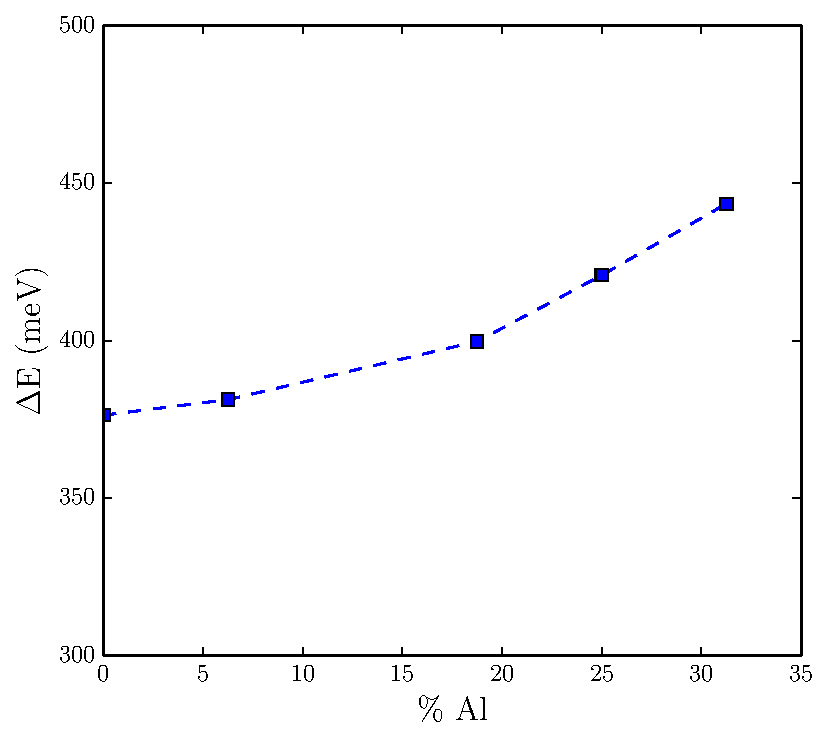
\includegraphics[scale=0.5]{figure_5a}
        \label{fig:Co_Al_dE_sn}
        }
    \subfigure[]{
     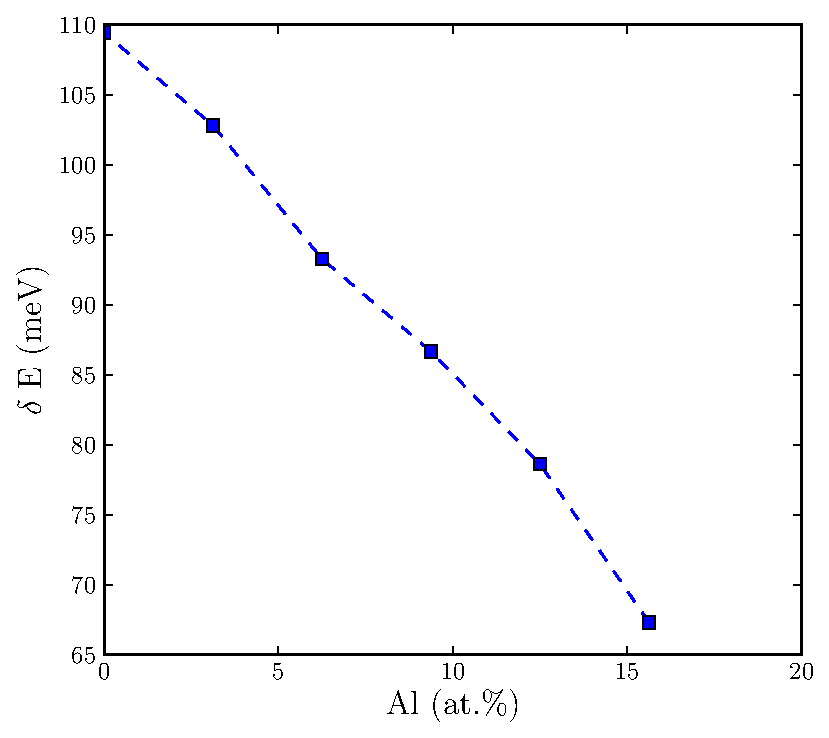
\includegraphics[scale=0.5]{figure_5b}
        \label{fig:Co_Al_dE_ren}
        }     
\caption{Energy barrier trend as a function of Al \%  for the a) SN and b) WL mechanisms}
\label{fig:energy_barrier}
  \end{figure}

\begin{figure}[htp!]%[!h]
    \centering
    \subfigure[]{
     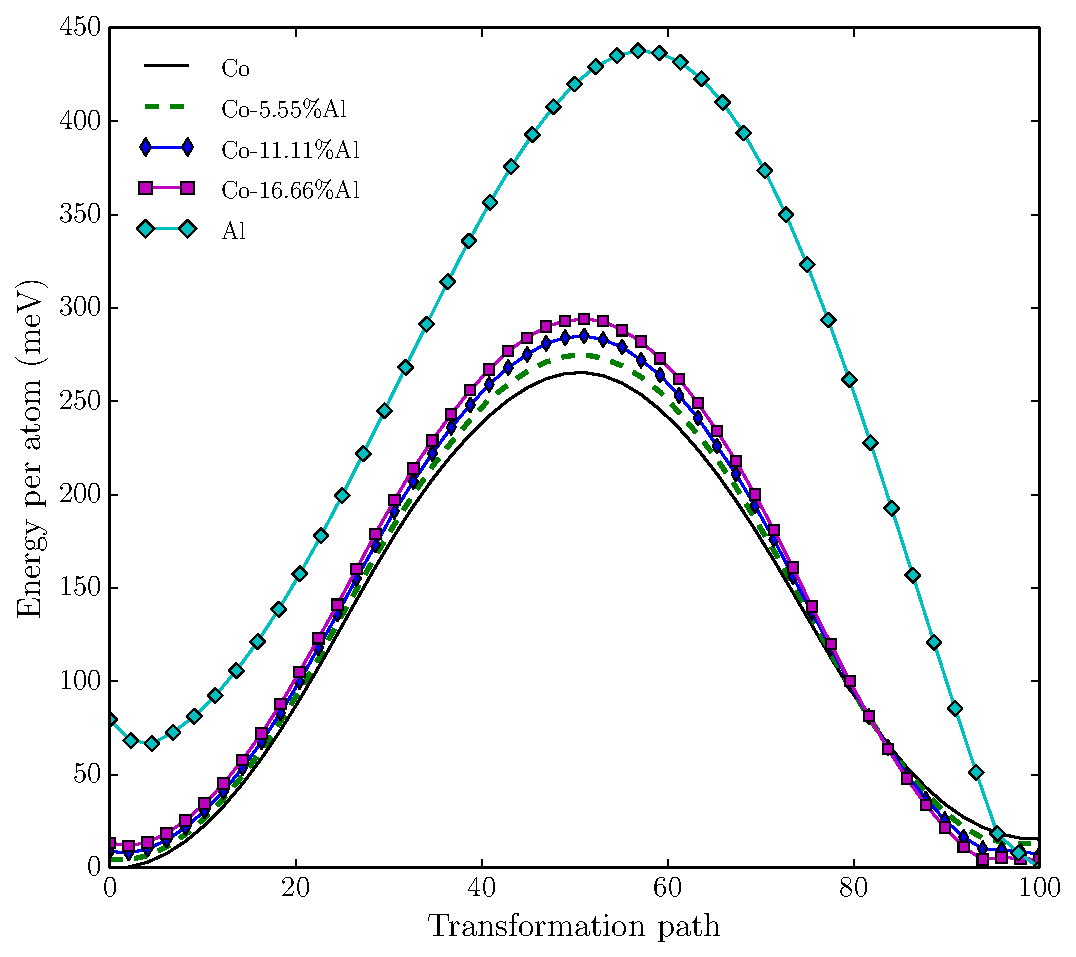
\includegraphics[scale=0.43]{figure_6a}
        \label{fig:Co_Al_sn_zero}
        }
  \subfigure[]{
        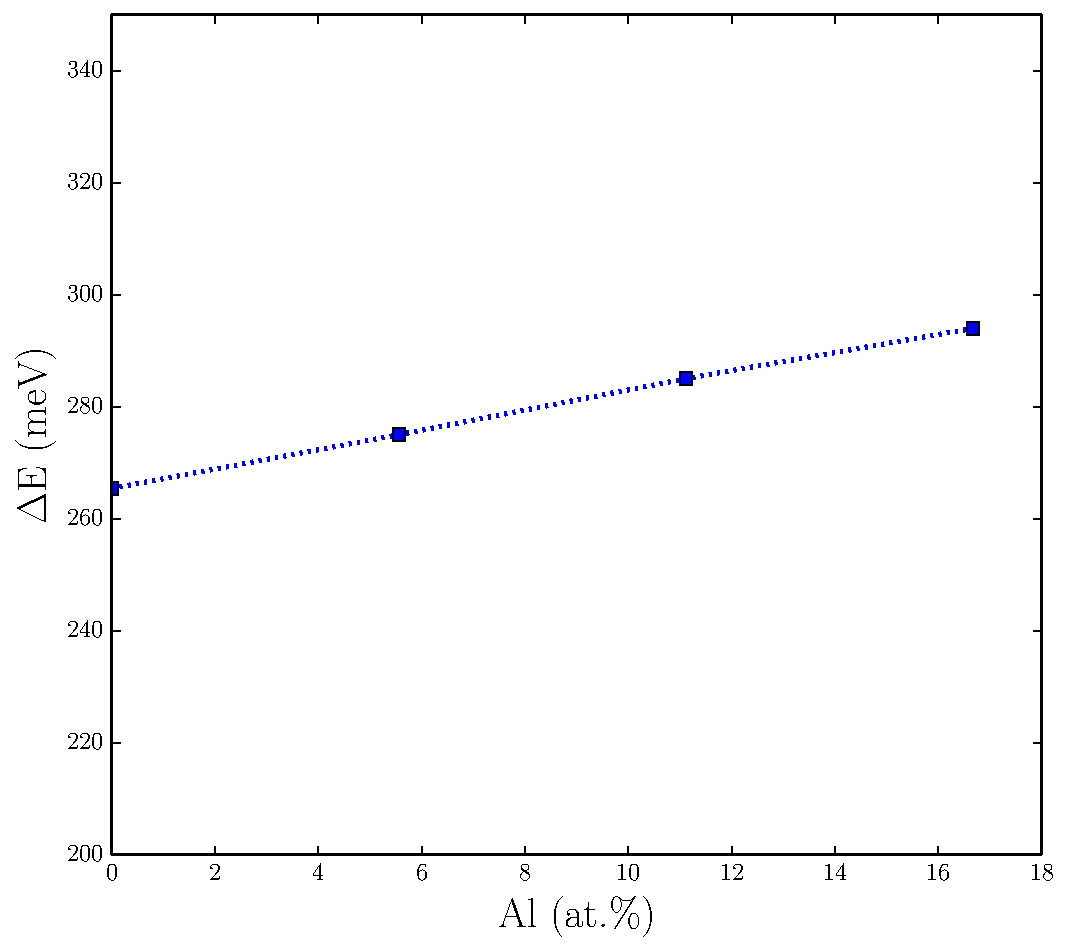
\includegraphics[scale=0.43]{figure_6b}
        \label{fig:Co_Al_dE_sn_zero}
        }
\caption{a) MEP profile for various compositions of Co - Al and b) Energy barrier trend as a function of Al \%  for the modified zero transformation shear SN mechanism}
\label{fig:modified_sn_zero}
  \end{figure}  

\begin{figure}[htp!]%[!h]
    \centering
    \subfigure[]{
     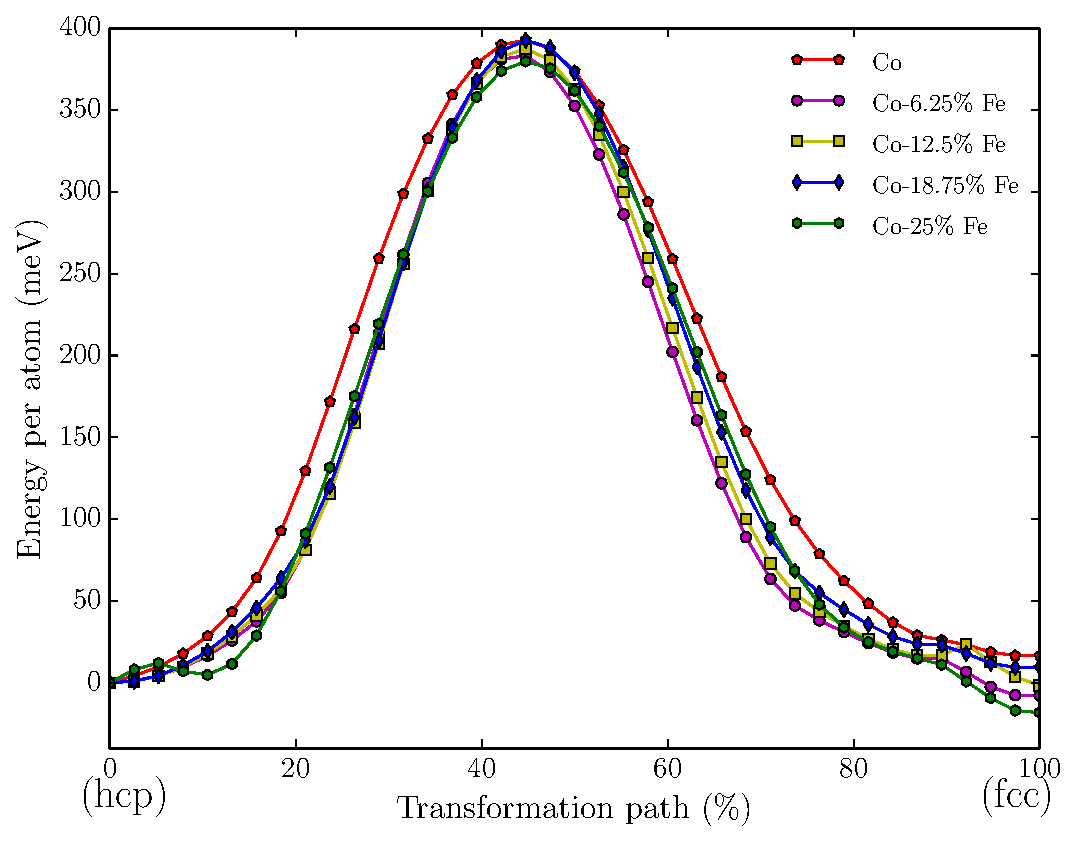
\includegraphics[scale=0.4]{figure_7a}
        \label{fig:Co_Fe_sn}
        }
  \subfigure[]{
        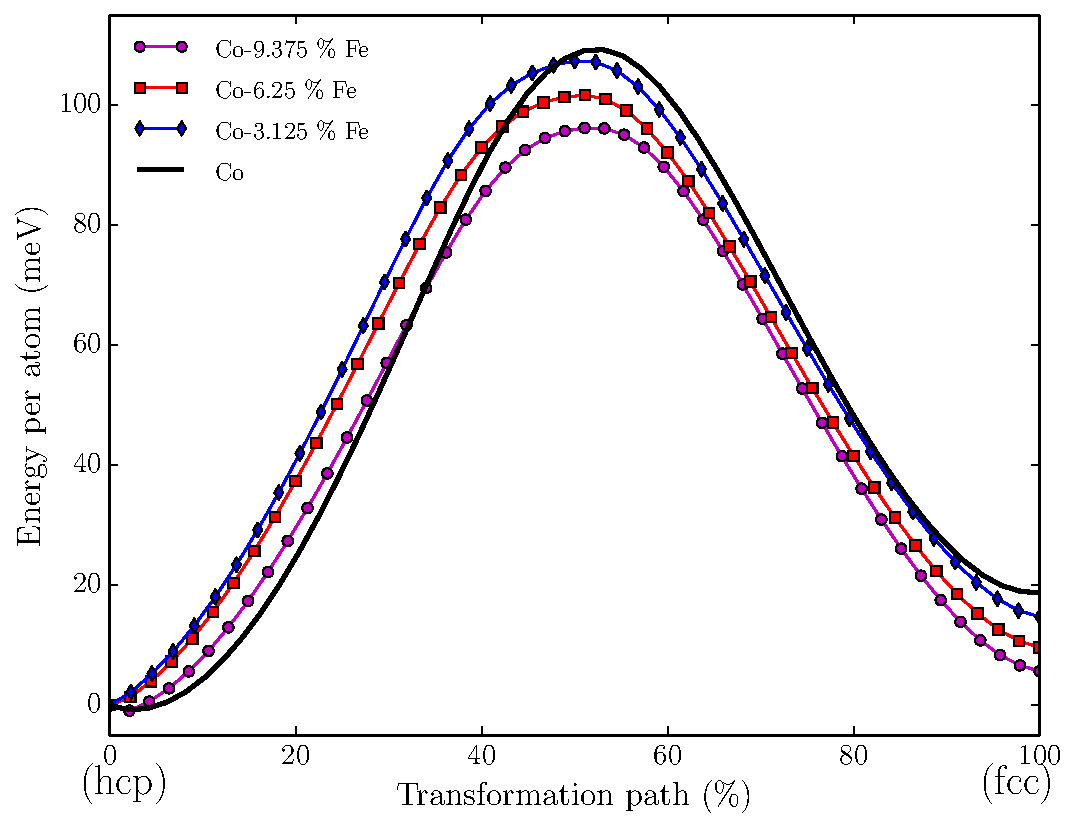
\includegraphics[scale=0.4]{figure_7b}
        \label{fig:Co_Fe_ren}
        }
\caption{MEP profile for various compositions of Co-Fe for the a) SN and b) WL mechanisms}
\label{fig:linear_profile_Co_Fe}
  \end{figure} 

\begin{figure}[htp!]%[!h]
    \centering
    \subfigure[]{
     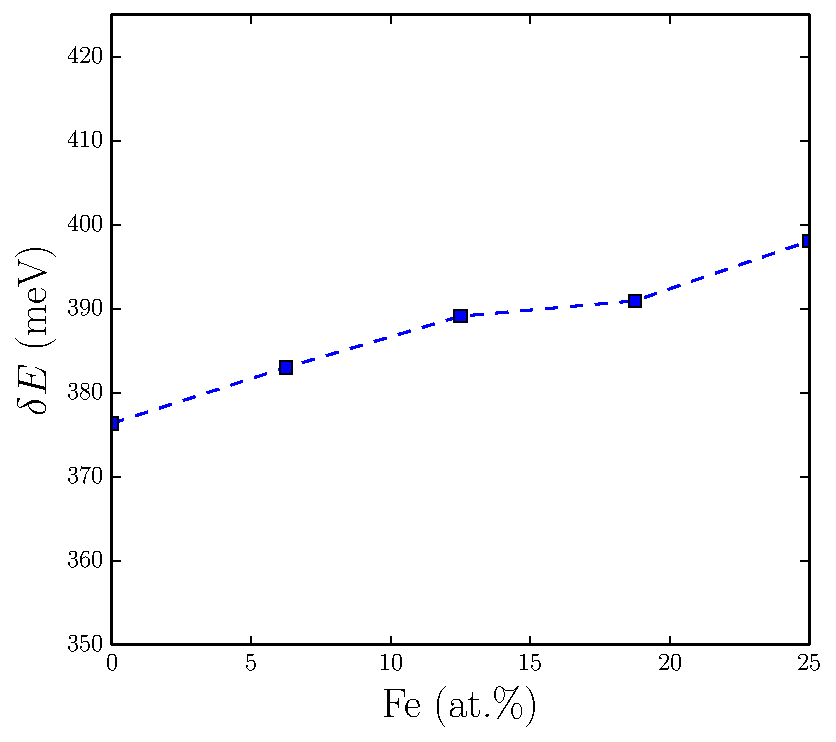
\includegraphics[scale=0.5]{figure_8a}
        \label{fig:Co_Fe_dE_sn}
        }
  \subfigure[]{
        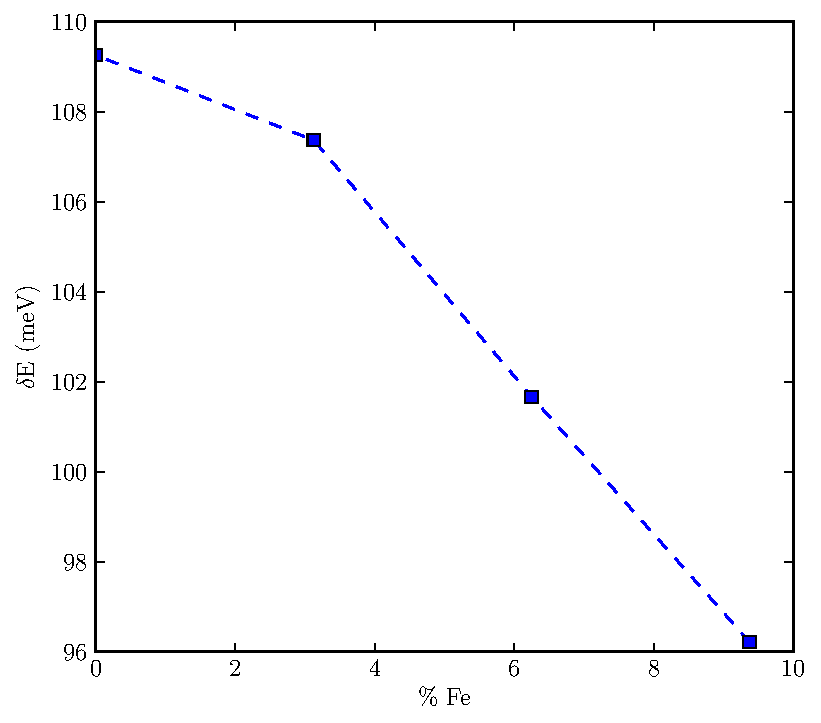
\includegraphics[scale=0.5]{figure_8b}
        \label{fig:Co_Fe_dE_ren}
        }
\caption{Energy barrier trend as a function of Fe \%  for the a) SN and b) WL mechanisms}
  \end{figure}
 
 Figure \ref{fig:Co_Fe_sn} shows the MEP profiles for varying compositions of Co-Fe  and Figure \ref{fig:Co_Fe_dE_sn} shows the trend observed in the energy barrier for the transformation for varying compositions of Co-Fe  for the Shoji-Nishiyama  model.
 Figure \ref{fig:Co_Fe_ren} shows the MEP profiles for varying compositions of Co-Fe   and Figure \ref{fig:Co_Fe_dE_ren} shows the trend observed in the energy barrier for the transformation for varying compositions of Co-Fe using the WL model. 
In the Co-Fe system , both models show  a reduction in the energy barrier (which indicates a lowering of $M_s$) for increasing amounts of Al, which corroborates experimental data \cite{ma2010high}.

\begin{figure}[htp!]%[!h]
    \centering
    \subfigure[]{
     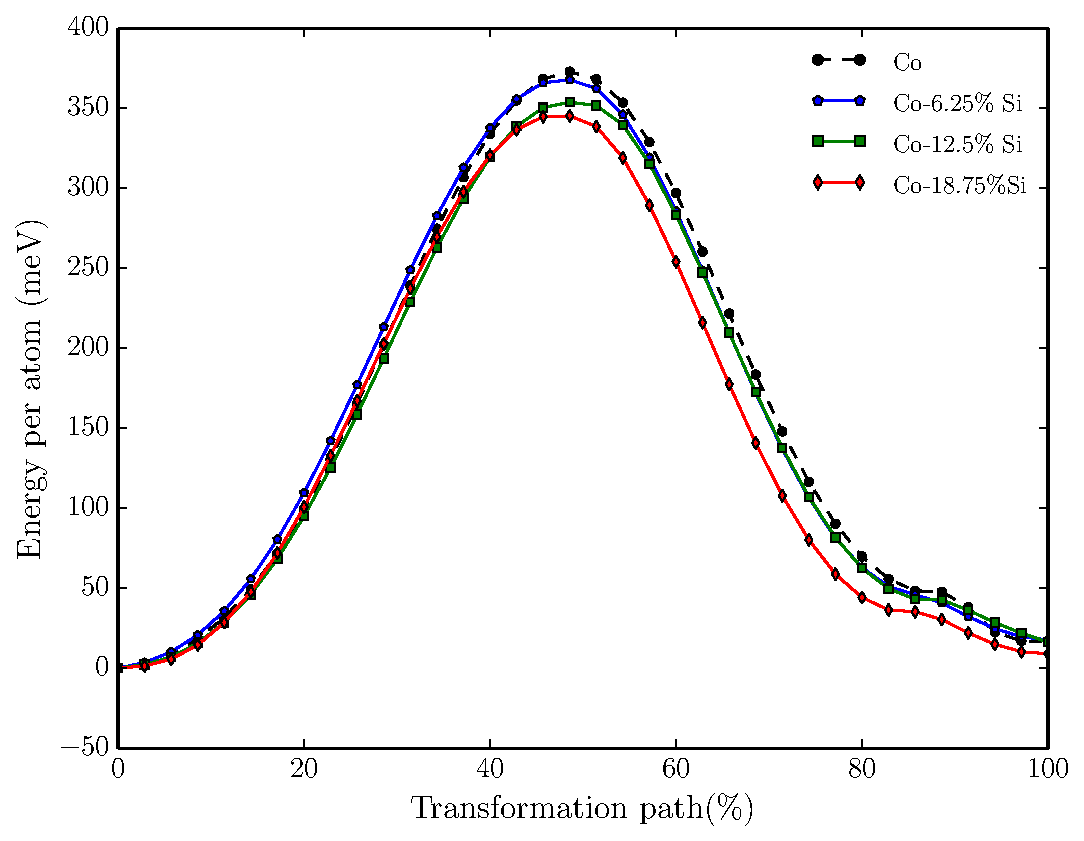
\includegraphics[scale=0.4]{figure_9a}
        \label{fig:Co_Si_sn}
        }
  \subfigure[]{
        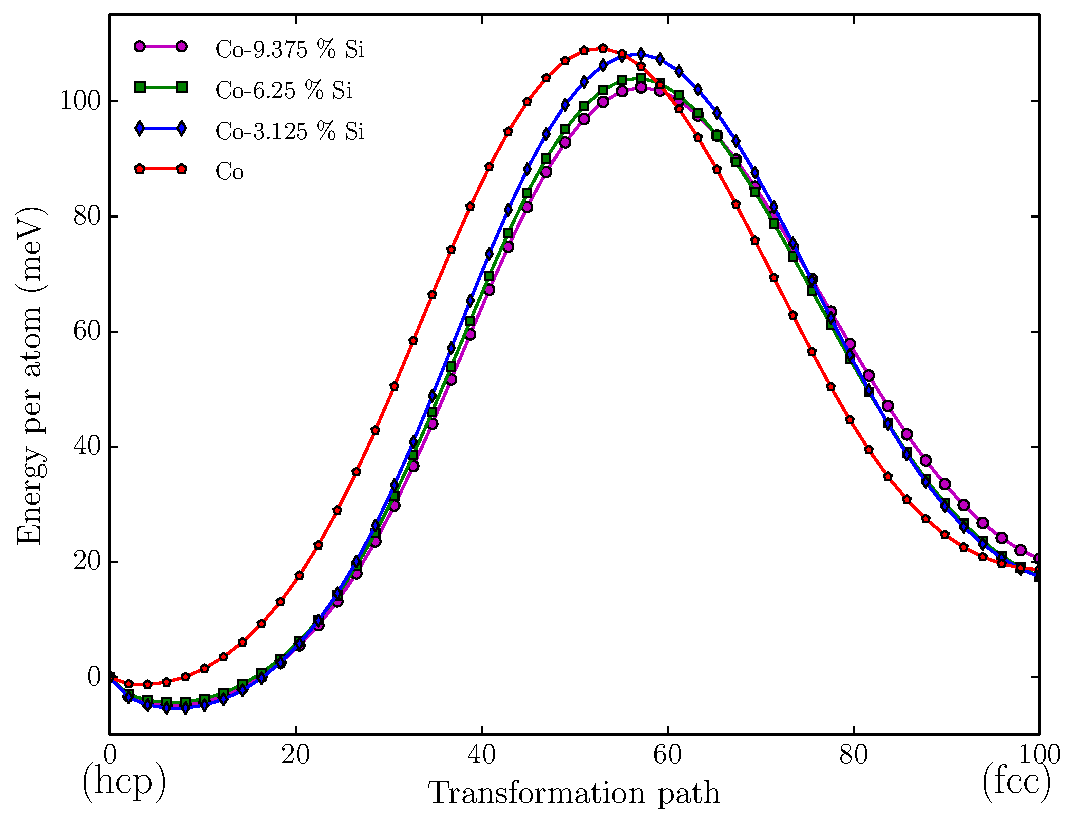
\includegraphics[scale=0.4]{figure_9b}
        \label{fig:Co_Si_ren}
        }
\caption{MEP profile for various compositions of Co-Si for the a) SN and b) WL mechanisms}
\label{fig:linear_profile_Co_Si}
  \end{figure}

\begin{figure}[htp!]%[htp]
    \centering
    \subfigure[]{
     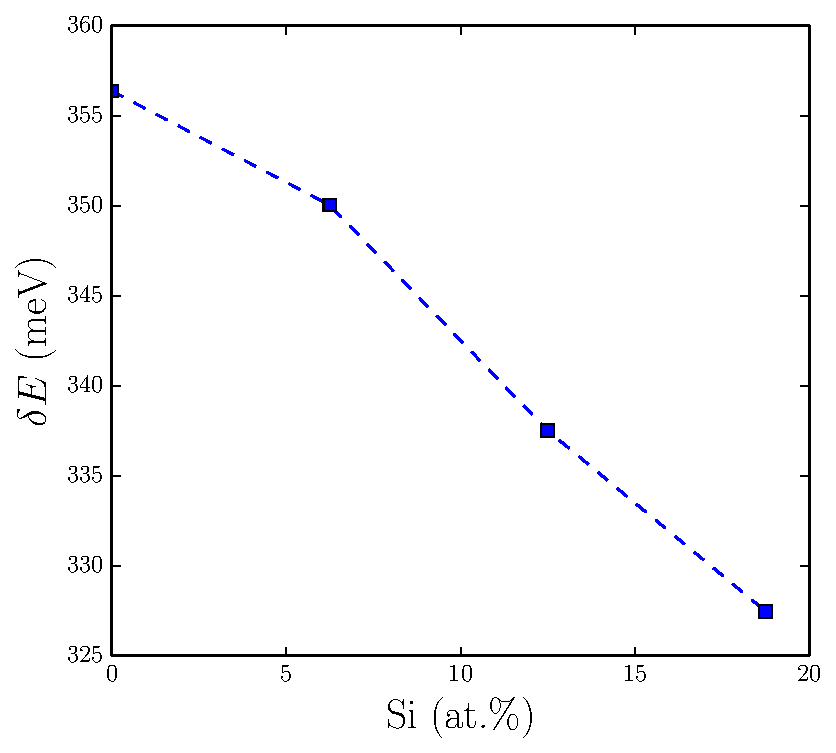
\includegraphics[scale=0.5]{figure_10a}
        \label{fig:Co_Si_dE_sn}
        }
  \subfigure[]{
        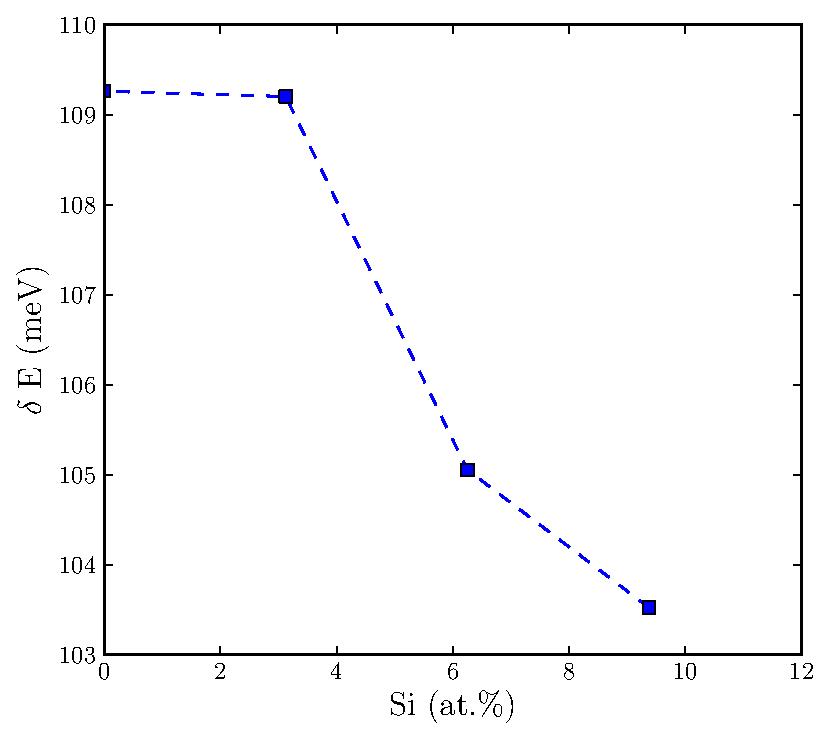
\includegraphics[scale=0.5]{figure_10b}
        \label{fig:Co_Si_dE_ren}
        }
\caption{Energy barrier trend as a function of Si \%  for the a) SN and b) WL mechanisms}
  \end{figure}
 Figure \ref{fig:Co_Si_sn} shows the MEP profiles for varying compositions of Co-Si  and Figure \ref{fig:Co_Si_dE_sn} shows the trend observed in the energy barrier for the transformation for varying compositions of Co-Si  for the Shoji-Nishiyama  model.
 Figure \ref{fig:Co_Si_ren} shows the MEP profiles for varying compositions of Co-Si   and Figure \ref{fig:Co_Si_dE_ren} shows the trend observed in the energy barrier for the transformation for varying compositions of Co-Si using the WL model. 
In the Co-Si system , both models show  a reduction in the energy barrier (which indicates a lowering of $M_s$) for increasing amounts of Si, which is contrary to what may be expected from experiments\cite{ma2010high}.

\textcolor{red}{Co being a magnetic element, it is possible that the magnetism may affect the transformation characteristics of the Co-based alloys. All calculations presented here are spin-polarized calculations. Non spin-polarized calculations were also carried out for the Co-Al alloys, but no significant difference was observed either qualitatively or quantitatively.}

Thus it is seen that the WL model predictions agree with experiments for the Co - Al and the Co-Fe systems. The SN mechanism calculations agree with experiments for the  Co-Fe system. Both mechanisms fail to explain the trends seen in Co-Si. It may therefore be possible, that the underlying energetics of the Co-Si system are far removed fom those of the Co - Al and Co-Fe systems. We propose that the martensitic transformation  in  Co - Al and Co-Fe may be explained by the Wentzcovitch -Lam  model.

While noting the MEP indicated by both mechanisms we see that the the MEP always passes through an intermediate structure and does not show the slightest tendency to deviate from the
intermediate structure. This can be explained on the basis of space group symmetry. A space group is a set of symmetry elements which always fulfill
certain conditions according to the mathematics of the particular group. If $G_n$ is a space group consisting of certain ’$n$’ symmetry
elements and $G_m$ is another space group with ’$m$’ symmetry elements such that $m \subseteq n$,then $G_m$ is the sub-group of $G_n$ while $G_n$ is the super-group of $G_m$. The martensitic 
transformation under consideration, is a barrier crossing event.  The transformation occurs from  the f.c.c structure to the h.c.p structure. F.c.c is a high symmetry structure with a space group
of 225 while h.c.p is a comparatively low symmetry structure (space group 194). Thus the transformation involves a reduction of symmetry. Reduction of symmetry happens through intermediate
common subgroup structures-transition states. This makes it necessary to used an optimization method to calculate the MEP. Not using a specific MEP method makes us overlook the
transition states which reflect the true mechanism of transformation. For f.c.c and h.c.p we see the common subgroup with the highest symmetry is the \textit{Cmcm} orthorhombic 
structure (space group:63). On examining the structure of the intermediate state indicated by the MEP, it is seen that it is the \textit{Cmcm} structure with a space group of 63.
%----------------------------------------------------------------------------------------------------------------------------------------------------------------------------------------------------------------------%
\section{Summary and Conclusion}
\label{Sec:summary}
The present work deals with the application of displacive transformation models to Co-based potential shape memory alloys. The f.c.c-b.c.c and f.c.c -h.c.p transformations have been modeled for the Co - Al and the Co - Al, Co-Fe, Co-Si systems respectively. The Bain path calculations for Co - Al showed an energy minimum at a
tetragonal structure upto 25 \% Al and indicated a theoretical possibility for the f.c.c - b.c.c transformation in Co - Al. The lack of a b.c.c phase in the cobalt phase diagram however, prohibits the expectation of this transformation in this system.
Two varied  parameterized models were used  to model the f.c.c - h.c.p
structural transformation for three Co-based SMA’s. The Wentzcovitch - Lam model predictions agree with experiments for the Co - Al and the Co-Fe systems. The Shoji-Nishiyama mechanism calculations agree with experiments for the  Co-Fe system. Both mechanisms fail to explain the trends seen in Co-Si. It may therefore be possible, that the underlying energetics of the Co-Si system are far removed from those of the Co - Al and Co-Fe systems. We propose that the martensitic transformation  in  Co - Al and Co-Fe may be explained by the Wentzcovitch - Lam  model. The intermediate structures obtained across both models for all the systems  conform to the common symmetry subgroup theory
%----------------------------------------------------------------------------------------------------------------------------------------------------------------------------------------------------------------------%
\section{Acknowledgements}
\label{Sec:ack}
R. Arr\'{o}yave and A. Talapatra acknowledge the support from NSF through grants CMMI-0953984, DMR-0805293 and DMR-DMR-0844082 (International Institute for Multifunctional Materials for Energy Conversion-IIMEC). First-principles calculations by RA and AT were carried out in the Chemical Engineering Cluster and the Texas A\& M Supercomputing Facility at Texas A\&M University as well as the Texas Advanced Computing Center (TACC) at the University of Texas-Austin. Preparation of the input files and analysis of the data have been performed within the framework  of AFLOW/ACONVASP developed by Stefano Curtarolo as well as with the ATAT package developed by Axel van de Walle.
\bibliographystyle{elsarticle-num}  
\bibliography{Co_Al}
\end{document}
